\documentclass[tikz,convert={outfile=\jobname.svg}]{standalone}

\begin{document}

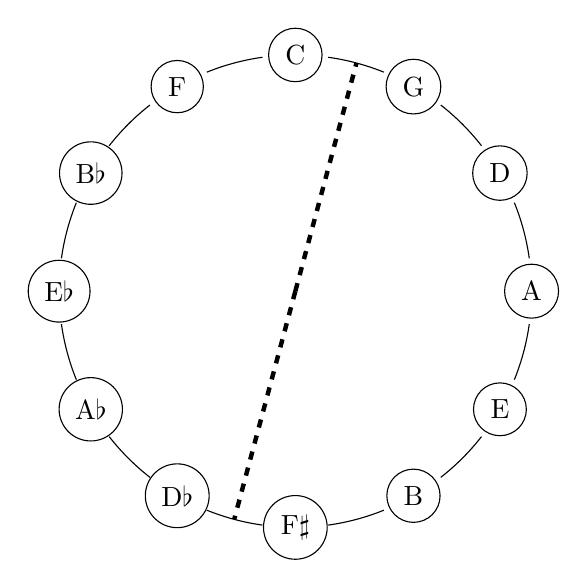
\begin{tikzpicture}

    \def \n {12}
    \def \radius {3cm}
    \def \margin {8} % margin in angles, depends on the radius
    
    \foreach \s/\key in {-5/D$\flat$, -4/A$\flat$, -3/E$\flat$, -2/B$\flat$, -1/F, 0/C, 1/G, 2/D, 3/A, 4/E, 5/B, 6/F$\sharp$}
    {
      \node[draw, circle] at ({90-360/\n * (\s)}:\radius) {\key};
      \draw[-, >=latex] ({360/\n * (\s - 1)+\margin}:\radius) 
        arc ({360/\n * (\s - 1)+\margin}:{360/\n * (\s)-\margin}:\radius);
    }

    \draw [ultra thick, dashed] (0, 0) --++ (75 : \radius);
    \draw [ultra thick, dashed] (0, 0) --++ (75 - 180:\radius);
\end{tikzpicture}

\end{document}




    % % \pgfmathsetmacro{\CircleRadius}{3.5}
    % % \pgfmathsetmacro{\LabelRadius}{\CircleRadius \* 0.9}
    
    % % \draw (0,0) circle (3.5);
    % % \foreach \X in {1, 2, 3, 4, 5, 7, 8, 9, 10, 11} {
    % %     % \draw (0,0) --++ (75 - \X \* 360 / 12 : 3.5);
    % %     \node[draw, circle] at (360 / 11 * \X)
    % % }

    % 
    % % OUTER LABELS  
    % % \foreach \X/\KeyText in {-5/D$\flat$, -4/A$\flat$, -3/E$\flat$, -2/B$\flat$, -1/F, 0/C, 1/G, 2/D, 3/A, 4/E, 5/B, 6/F$\sharp$}
    % % {
    %     % \draw (90-\X\*360/12:\LabelRadius) node {\KeyText};
    % % }